% Corrected version (2026-10-27) of Generating_Secure_And_Quality_Code.pdf.
% Framing: updated measurement study (RQ1, reported) + design proposal with an
% evaluation plan (RQ2-RQ6, future work). Every RQ1 number was checked against
% evaluation/results/* (see work_log.md step 19). Do not edit numbers by hand.
\documentclass[conference]{IEEEtran}
\IEEEoverridecommandlockouts
\usepackage{cite}
\usepackage{amsmath,amssymb,amsfonts}
\makeatletter
\IfFileExists{algorithm.sty}{\usepackage{algorithm}}{%
  % Fallback for TeX installations without the algorithms bundle.
  \newcounter{algorithm}
  \def\fps@algorithm{tbp}\def\ftype@algorithm{4}\def\ext@algorithm{loa}
  \def\fnum@algorithm{Algorithm~\thealgorithm}
  \newenvironment{algorithm}{\@float{algorithm}}{\end@float}}
\makeatother
\IfFileExists{algorithmic.sty}{\usepackage{algorithmic}}{%
  % Minimal fallback covering only the commands used in Algorithm 1.
  \newcounter{algline}\newlength{\algind}
  \newenvironment{algorithmic}[1][0]{\begin{list}{\footnotesize\arabic{algline}:}%
    {\usecounter{algline}\setlength{\leftmargin}{1.8em}\setlength{\itemsep}{0pt}%
     \setlength{\parsep}{0pt}\setlength{\algind}{0pt}}}{\end{list}}
  \newcommand{\algln}{\item\hspace*{\algind}}
  \newcommand{\STATE}{\algln}
  \newcommand{\REQUIRE}{\item[]\textbf{Require:} }
  \newcommand{\RETURN}{\algln\textbf{return} }
  \newcommand{\TO}{\textbf{to}\ }
  \newcommand{\OR}{\ \textbf{or}\ }
  \newcommand{\FOR}[1]{\algln\textbf{for} ##1 \textbf{do}\addtolength{\algind}{1em}}
  \newcommand{\FORALL}[1]{\algln\textbf{for all} ##1 \textbf{do}\addtolength{\algind}{1em}}
  \newcommand{\ENDFOR}{\addtolength{\algind}{-1em}\algln\textbf{end for}}
  \newcommand{\IF}[1]{\algln\textbf{if} ##1 \textbf{then}\addtolength{\algind}{1em}}
  \newcommand{\ENDIF}{\addtolength{\algind}{-1em}\algln\textbf{end if}}}
\usepackage{graphicx}
\usepackage{textcomp}
\usepackage{xcolor}
\usepackage{booktabs}
\usepackage{tikz}
\usetikzlibrary{arrows.meta,positioning,fit,calc}

% Symbols for the positioning table
\newcommand{\yes}{\checkmark}
\newcommand{\prt}{$\circ$}
\newcommand{\no}{--}

\begin{document}

\title{Generating Secure and High-Quality Code with LLMs by Combining CWE
Vulnerability Knowledge and Business Logic Understanding: An Updated
Measurement and a Framework Design}

% TODO(authors): university name, city and emails are still placeholders.
\author{
\IEEEauthorblockN{
Manda Bharath Kumar,
Dileep Yarrabothula,
Sai Prakash Avula,
Dr. M Venu Gopalachari
}
\IEEEauthorblockA{
\textit{Department of Information Technology} \\
\textit{University Name} \\
City, India \\
email1, email2, email3, email4
}
}

\maketitle

\begin{abstract}
Large language models now write a growing share of production code, yet
measurement studies show that the code they produce repeatedly carries
language-specific weaknesses. We first update a recent multi-language
measurement study with five current lower-cost models on 800 combinations of
task, model and language (40 tasks, four languages). Of these, 75.5\%
produced complete code that parses and compiles; 15.9\% of those artifacts
carried at least one medium- or high-severity scanner finding, concentrated in
C; and the base study's functional tests that we could approve for reuse
covered only 16.2\% of combinations and checked no security property. Existing
tests and scanners therefore cannot by themselves establish whether generated
code enforces its security requirements. Together with recent evidence that
models know secure-coding rules but fail to apply them, that static analyzers
overstate security, that authorization flaws are invisible to pattern-based
tools, and that security degrades across edits, this motivates the second part
of the paper: the design of a framework that treats the \emph{location} of
enforcement as a first-class object. The framework compiles CWE-derived
mitigations and developer-confirmed business rules, such as ownership, role
permissions and workflow invariants, into typed obligations and binds each
obligation to a named slot in a code skeleton before any implementation is
written. A generated security test is trusted only after it fails on a
weakened version of its own slot, repair is confined to the failing slot, and
validated tests are kept as a regression ledger across later features. We
define the metrics, baselines and ablations for evaluating the framework;
implementing and evaluating it is the subject of follow-up work.
\end{abstract}

\begin{IEEEkeywords}
Large Language Models, Secure Code Generation, Common Weakness Enumeration,
Business Logic, Authorization, Mutation Testing, AI-Assisted Software
Development
\end{IEEEkeywords}

%==========================================================================
\section{Introduction}
%==========================================================================

Large language models (LLMs) have moved from completing lines of code to
writing whole features and, through conversational ``vibe coding''
workflows, whole applications. This changes where the cost of a defect
falls. A developer no longer reviews logic they wrote; they review logic an
assistant wrote, often faster than they can verify it. Controlled studies
suggest the cost is real: participants with an AI assistant wrote less
secure code while being more confident it was secure \cite{perry2023}, and
experienced open-source developers in a randomized trial were 19\% slower
with AI assistance while believing they were 20\% faster, spending part of
their time reviewing and cleaning AI output \cite{metr2025}. As generation
becomes cheaper and review does not, the effort needed to establish that
generated code is safe becomes the limiting factor. Reducing that effort,
rather than only reducing vulnerability counts, is the practical problem this
work addresses.

The underlying weakness is well documented. Kharma \textit{et al.} measured
five LLM families on 200 tasks in four languages and found recurring,
language-specific weaknesses, with cryptographic misuse such as RSA without
OAEP (CWE-780), hardcoded passwords (CWE-259) and improper certificate
validation (CWE-295) prominent in Java and Python, and buffer errors such as
CWE-120 in C \cite{kharma2026}. Agent benchmarks show the same pattern at
larger scale. On real-world feature tasks, the best agent configuration in
SusVibes passed functional tests on 61.0\% of tasks but was also secure on
only 10.5\% \cite{susvibes2026}, and on exploit-tested backend tasks roughly
half of functionally correct programs were exploitable \cite{baxbench2025}.

Three findings explain why existing mitigations struggle. First, knowledge
is not the bottleneck: across eighteen model and benchmark slices, models
answered secure-coding questions with 93.7--96.5\% accuracy, yet the gap
between knowledge and secure generation was 47.9 points on CWEval and 72.9
points on BaxBench \cite{sok2026}. Methods that retrieve more CWE guidance
into the prompt \cite{securecoder2026,macot2026,csdd2026} therefore address
the part of the problem that is already largely solved. Second, the
checkers used to measure progress are unreliable: CodeQL rated 64.8--98.5\%
of outputs from secure-generation methods as secure while only
3.0--13.3\% were both secure and functional \cite{tessa2026}, and
static analyzers cannot see a missing ownership check at all, because there
is no source-to-sink pattern for ``this user must not see that order.''
Third, security is not stable over time: correct-and-secure rates fall by
20--27\% when tasks are spread over multiple turns \cite{mtsec2025}, and
feature-adding steps were the most likely to degrade security in long
refinement chains \cite{scaffold2026}.

Business logic sits at the intersection of these problems. The closest work,
a specification-driven pipeline that derives a multilayer security model
from business and technical specifications, reduced business-logic test
failures from 17 to 9 on a booking API, but never executed its own
verification layer \cite{specdriven2026}; a CWE-tagged constitution approach
explicitly leaves business-logic flaws out of scope \cite{csdd2026}. Repair
loops add their own failure mode: methods that iterate until a checker is
satisfied often do so by deleting or breaking functionality
\cite{dai2025,sok2026}.

This paper has two parts. The first is an updated measurement: we re-run the
base study's setting \cite{kharma2026} on 40 of its tasks with five current
lower-cost models and pass every output through the same deterministic gate,
sandboxed tests and scanners. The measurement shows directly that the tests
and scanners available for such code say little about whether it enforces its
security requirements. The second part takes the position that the missing
element is the \emph{location} of enforcement. A requirement such as ``only
the owner may cancel a booking'' is satisfied only if a check exists at one
specific place on the request path, before the state change. We propose a
framework that makes that place a first-class object. It compiles CWE-derived
mitigations and developer-confirmed business rules into typed
\emph{obligations}, and binds each obligation to a named \emph{slot} in a code
skeleton before implementation begins, following the spirit of Design by
Contract \cite{meyer1992}. The binding is then used three ways. A generated
security oracle is trusted only if it fails when its own slot is replaced by a
permissive mutant, giving every test built-in evidence that it can detect the
flaw it targets. Repair of a failing obligation may edit only the
corresponding slot. Validated oracles are committed with the code as a ledger
and must remain green as later features are added. Each obligation ends as
PASS, FAIL, or WAIVED, so a reviewer reads a short list of what was not proven
rather than every generated line. This paper presents the design and its
evaluation plan; the implementation and its results will be reported
separately.

The contributions of this work are:
\begin{itemize}
\item \textbf{An updated measurement.} An updated, partial re-measurement of
the base study on 800 combinations of 40 tasks, five current lower-cost
models and four languages, with a deterministic completeness and compilation
gate, sandboxed functional testing, multi-tool scanning, paired statistics, a
descriptive comparison with the base study's published outputs and a
disjoint-task check (Section~III).
\item \textbf{Slot-bound security contracts (design).} A typed obligation
schema that unifies CWE-derived and business-context requirements, each with a
source, severity, slot and verifier kind, together with a skeleton-first
binder and a static check that every route reaches its bound guards.
\item \textbf{Mutation-validated invariant oracles (design).} Deterministic
generation of multi-identity authorization and workflow oracles from a
confirmed access matrix, with slot-targeted mutation that makes oracle
adequacy a reported quantity and separates ``waived'' from ``passed.''
\item \textbf{Slot-scoped repair, a defense-survival protocol and an
evaluation plan.} A repair step that cannot modify code outside the failing
slot, a metric for how many validated defenses survive each added feature,
and a controlled evaluation design with joint functional and security
metrics against strong agentic, specification-based and repair baselines.
\end{itemize}

Section~II reviews related work. Section~III reports the updated measurement
(RQ1) and what it implies for the design. Section~IV defines the problem,
threat model, metrics and research questions. Section~V presents the
framework, and Section~VI the plan for evaluating it. Section~VII discusses
threats to validity and Section~VIII concludes.

%==========================================================================
\section{Related Work}
%==========================================================================

\subsection{Measuring the Security of Generated Code}

Kharma \textit{et al.} \cite{kharma2026} provide the measurement baseline
this work extends: a curated 200-task dataset in seven categories, four
languages and five model families, evaluated for compilation, unit-test
correctness, and quality and security with SonarQube and CodeQL. Perry
\textit{et al.} \cite{perry2023} showed in a user study that assistance can
lower security while raising confidence. Later work moved to executable
evaluation. BaxBench pairs 392 backend tasks with expert exploits and found
the best correct-and-secure rates around 35--37\% \cite{baxbench2025};
CWEval provides function-level tasks with executable functional and security
tests \cite{cweval2025}; SusVibes and an independent re-run by Endor Labs
evaluate agents on repository-level feature tasks, where pooled across
thirteen agent and model pairs 90.5\% of tasks were solved functionally but
only 33.0\% securely \cite{susvibes2026,endor2026}.

These studies also expose evaluation pitfalls that shape our design. Static
verdicts overstate security by 7.4--21.6 times relative to combined static
and functional checks \cite{tessa2026}, and on 1,080 human-labelled samples
Semgrep and CodeQL agreed with human judgement on only 65\% and 61\% of
samples \cite{sastlabels2026}. Agents also find shortcuts: in one SusVibes
run, an agent recovered known fixes from git history in 163 of 200 tasks
\cite{endor2026}. The framework therefore uses executable oracles as the
primary security measure, treats static findings as secondary, and isolates
the sandbox from network and version history.

\subsection{Steering Generation with Vulnerability Knowledge}

A large family of methods adds security knowledge at inference time.
SecureCoder maps a task to CWE descriptions and derives guidelines
\cite{securecoder2026}; MA-CoT retrieves task-specific CWE mitigations into
a chain-of-thought prompt and was evaluated on the base paper's dataset with
static tools and manual review \cite{macot2026}; BRACE uses an LLM to
identify task-relevant CWE risks and validates them against the CWE catalog
\cite{brace2026}; Constitutional Spec-Driven Development (CSDD) encodes
CWE-tagged principles with MUST/SHOULD levels and reports CWE violations
falling from 11 to 3 on a single application, with targeted principles
outperforming the full set \cite{csdd2026}. The systematization by Patir
\textit{et al.} explains why such gains are bounded: models already know the
principles, and the gap lies in applying them at the right place
\cite{sok2026}. Among its recommended directions are sink-grounded guidance
and localized, function-preserving repair, neither of which it found
implemented. CSDD comes closest by producing a file-and-line traceability
matrix, but the matrix is produced with or after implementation and, in the
authors' words, measures documented traceability rather than security
effectiveness \cite{csdd2026}. The proposed framework instead binds
obligations before implementation and ties each binding to an executable,
validated oracle.

\subsection{Execution Feedback, Agents and Repair}

Executing code is a strong baseline. In the same systematization, an agent
scaffold with no security component raised secure-pass@1 on CWEval from 60.5
to 91.6 for one model, but only from 34.2 to 41.8 on the multi-endpoint
BaxBench tasks \cite{sok2026}. SCGAgent generates unit tests, predicts
likely CWEs and applies guidelines with re-testing; it improved one model
but degraded others because self-generated tests were unreliable, and its
CWE prediction recall was 0.448 \cite{scgagent2025}. Supplying security
tests to the model as an upfront specification improved results by 19.3
points on 31 Python tasks, but the tests were benchmark-provided, did not
cover authorization, and repair required replacing the whole module
\cite{testsasspec2026}. A static-analysis feedback loop using Bandit, Pylint
and CodeQL lowered the insecure rate from about 43--45\% to 13.41\% while
improving correctness \cite{blyth2025}. Repair loops also over-correct: an
independent re-evaluation found that 10--30\% of tasks solved by base models
broke after applying secure-generation methods, with one method resolving
most failures by deleting the vulnerable code \cite{dai2025}. LLM-written
exploits are unreliable unless validated by execution: 44--71.5\% of
proof-of-concept exploits that agents counted as successful were invalid
\cite{pocgym2026}, whereas requiring an exploit to fail on a secure solution
and succeed on a weakened one yielded 96.77\% expert-rated soundness
\cite{autobax2025}. The framework adopts this contrastive idea but obtains the
weakened variant by mutating the bound slot, which does not require a
reference solution.

\subsection{Business Logic, Specifications and Authorization}

Grynets \textit{et al.} \cite{specdriven2026} propose a Multilayer
Specification Security Model covering actors, roles, assets, trust
boundaries and ownership, fed to an agent through GitHub Spec Kit. On a
FastAPI booking API with a hidden 221-test suite, total failures fell from 50
without security requirements to 42 with ASVS conditioning and 36 with their
model, and business-logic failures fell from 17 to 9. The authors list
executing the verification scenarios, mapping requirements to code,
post-generation repair and multi-turn work as future work; these are the
gaps the framework targets. LLM threat elicitation remains only moderately
accurate: the same pipeline fully covered 45.45\% of reference threats
\cite{specdriven2026}, and open 8B models peaked at 68.75\% penalized F1 on
STRIDE classification \cite{threatmodel2026}. AutoCedar shows how to make
intent reliable: humans approve must-permit and must-deny boundaries, after
which a solver-guided loop produced verified Cedar policies for all 221
tasks \cite{autocedar2026}. Automated broken object-level authorization
(BOLA) detection with multiple identities exists for deployed APIs
\cite{authprobe2026}, but covers read access on existing services rather than
generated code. The framework combines these ideas: the developer confirms an
access matrix, and oracles for both read and write operations are generated
from it deterministically.

\subsection{Security Across Turns}

MT-Sec measured a 20--27\% relative drop in correct-and-secure rate from
single-turn to multi-turn tasks, with a control showing the drop is not
explained by context length, and found that feedback from ground-truth tests
recovered most of the loss \cite{mtsec2025}. SCAFFOLD-CEGIS found that
feature-enhancement steps degraded security in 52.8\% of cases, that adding
static-analysis gating alone increased latent degradation from 12.5\% to
20.8\%, and that semantic anchors with diff budgets reduced degradation to
2.1\% \cite{scaffold2026}. EvoCode-Bench reports functional regression as a
leading failure mode for strong agents but does not score security
\cite{evocode2026}. The framework replaces static counts with executable,
validated oracles that persist across turns, and constrains repair by slot
rather than by diff size.

\subsection{Training-Based Methods}

Training approaches fine-tune models on secure and insecure pairs, use
preference optimization, or apply reinforcement learning with security
rewards \cite{srcode2026,secvec2026}, and constrained decoding restricts
generation to avoid known-insecure patterns \cite{codeguardplus2024}. Their
security signals come mostly from static analyzers or teacher models, which
inherit the checker problems above. We treat training as future work and
note that the framework would produce data, oracle-labelled slot repairs,
that could serve as an executable reward signal.

\subsection{Positioning}

Table~\ref{tab:positioning} summarizes how the proposed design relates to the
closest prior work. No single mechanism is new in isolation; the contribution
is binding obligations to slots before implementation and using that binding
to validate oracles, localize repair and attribute regressions. The last row
describes the design, not measured results.

\begin{table*}[t]
\caption{Positioning against the closest prior work (\yes{} = yes,
\prt{} = partial, \no{} = no)}
\label{tab:positioning}
\centering
\small
\begin{tabular}{@{}lccccccc@{}}
\toprule
\textbf{Work} & \textbf{Business} & \textbf{CWE} & \textbf{Executed} &
\textbf{Oracles} & \textbf{Pre-impl.} & \textbf{Localized} &
\textbf{Multi-turn} \\
 & \textbf{context} & \textbf{knowledge} & \textbf{oracles} &
\textbf{validated} & \textbf{binding} & \textbf{repair} &
\textbf{regression} \\
\midrule
MA-CoT \cite{macot2026} & \no & \yes & \no & \no & \no & \no & \no \\
CSDD \cite{csdd2026} & \no & \yes & \no & \no & \prt{}$^a$ & \no & \no \\
Spec-driven SDD \cite{specdriven2026} & \yes & \yes & \no$^b$ & \no & \no & \no & \no \\
Tests as spec \cite{testsasspec2026} & \no & \yes & \yes & \no & \no & \no & \no \\
SCGAgent \cite{scgagent2025} & \no & \yes & \yes & \no & \no & \no & \no \\
SCAFFOLD-CEGIS \cite{scaffold2026} & \no & \prt & \prt & \no & \prt{}$^c$ & \prt{}$^d$ & \yes \\
AutoBaxBuilder$^e$ \cite{autobax2025} & \no & \yes & \yes & \yes & \no & \no & \no \\
\midrule
This work (proposed design) & \yes & \yes & \yes & \yes & \yes & \yes & \yes \\
\bottomrule
\multicolumn{8}{@{}p{0.95\textwidth}@{}}{\footnotesize
$^a$Traceability matrix produced with or after implementation.
$^b$Hidden evaluation suite only; the method's verification layer is not
executed. $^c$Anchors mined from existing code. $^d$Diff-size budget rather
than location. $^e$Benchmark construction rather than a generation
method; validation uses a reference solution.}
\end{tabular}
\end{table*}

%==========================================================================
\section{Updated Measurement (RQ1)}
\label{sec:rq1}
%==========================================================================

RQ1 asks how complete, secure and maintainable code from current lower-cost
LLMs is across four languages, and how it compares with the base study
\cite{kharma2026}.

\subsection{Setup}

\textbf{Tasks, models and generation.} We use 40 tasks from the base study's
dataset, chosen by judgment within its task strata rather than at random, in
Python, Java, C and C++. We use five current lower-cost models accessed
through OpenRouter: Claude Haiku~5.5, GPT-6~Luna, Gemini~3.8 Flash, Mistral
Large~4 and Qwen3.8 Flash. This gives 800 planned combinations of task, model
and language. Each combination receives one sample at temperature 0.2, top-p
0.95 and at most 4,096 output tokens, with up to three attempts when the
response is empty, refused or invalid. The prompt is ours, not the base
study's, and the temperature differs from the base study's 0.9; both are
deviations we account for when comparing with the base study. All generated
artifacts are frozen in a snapshot with per-file hashes, and every later
stage verifies those hashes, so all results refer to the same code.

\textbf{Gate 1: completeness and compilation.} A deterministic gate that never
executes code checks integrity (empty output, truncation reported by the
provider, leftover Markdown fences), syntax (Python parsing and compilation,
Java parsing), and build (javac 21 for Java; clang 20.1.2 for C and C++,
compiled to object files without linking). Code that fails only because a
third-party header such as OpenSSL or libpq is missing is labelled
\emph{blocked} rather than counted as a model error. Passing the gate makes
an artifact eligible for testing and scanning; it is not evidence of
correctness.

\textbf{Functional tests.} We reuse the base study's published unit tests,
fetched at pinned commits, so that the oracle is independent of us. For each
task and language, a reference test is chosen and reviewed; name-only
adapters rebind function names without changing inputs or expected values.
Tests run in an isolated sandbox built with bubblewrap: no network, unshared
namespaces, dropped capabilities, a read-only root, and limits on time, CPU,
memory, processes and file size, verified by a 31-check self-test before
every batch.

\textbf{Security and quality analysis.} All artifacts are scanned with one
fixed configuration: Semgrep 1.182.1 with CWE Top 25 and security-audit rule
packs pinned by hash, Bandit 1.9.4 for Python, and Flawfinder 2.0.20 for C
and C++. Severities are mapped to low, medium and high, and the headline rate
counts artifacts with at least one medium- or high-severity finding, so one
noisy file cannot dominate. Quality is measured with Lizard 1.24.3 (lines of
code inside functions, cyclomatic complexity, and complexity density as
defined by the base study) and Cppcheck 2.13.0 for C and C++ reliability
defects. A sample of 65 findings is triaged to estimate how many are real.

\textbf{Statistics.} Rates carry Wilson 95\% intervals \cite{wilson1927}.
Models are compared in pairs with the exact McNemar test \cite{mcnemar1947}
on the 160 task and language cells both models attempted, which cancels
shared task difficulty, with Holm correction over the ten pairs
\cite{holm1979} and Newcombe intervals for paired differences
\cite{newcombe1998}. Every number in this section is computed by script from
row-level result files.

\textbf{Comparison with the base study's outputs.} The base study's 600
published C, C++ and Python files for the same 40 tasks are passed, byte for
byte, through the same gate and scanners. Java is excluded because no Java
outputs were published. Because models, prompt, temperature, token limits and
generation dates all differ, this comparison describes two cohorts of code
and supports no claim about individual models.

\begin{table}[t]
\caption{Gate 1 outcomes by model (160 combinations each)}
\label{tab:gate1}
\centering
\small
\setlength{\tabcolsep}{3pt}
\begin{tabular}{@{}lrrrrrr@{}}
\toprule
Model & Pass & Rate \% [95\% CI] & Inc. & Block. & Err. & None \\
\midrule
GPT-6 Luna & 134 & 83.8 [77.3, 88.7] & 11 & 14 & 1 & 0 \\
Gemini 3.8 Flash & 131 & 81.9 [75.2, 87.1] & 14 & 11 & 0 & 4 \\
Mistral Large 4 & 122 & 76.3 [69.1, 82.2] & 19 & 7 & 1 & 11 \\
Claude Haiku 5.5 & 118 & 73.8 [66.4, 80.0] & 31 & 8 & 2 & 1 \\
Qwen3.8 Flash & 99 & 61.9 [54.2, 69.0] & 10 & 1 & 0 & 50 \\
\midrule
All & 604 & 75.5 [72.4, 78.4] & 85 & 41 & 4 & 66 \\
\bottomrule
\multicolumn{7}{@{}p{0.97\columnwidth}@{}}{\footnotesize Inc.: incomplete,
truncated at the output limit or left in Markdown fences. Block.: failed only
because a third-party header is missing. Err.: syntax or compile error.
None: no artifact after all attempts.}
\end{tabular}
\end{table}

\begin{table}[t]
\caption{Results by language (200 combinations each)}
\label{tab:lang}
\centering
\small
\begin{tabular}{@{}lrrr@{}}
\toprule
Language & Gate 1 pass & $\geq$1 medium/high & Mean \\
 & & finding (of passes) & CCN \\
\midrule
Python & 186 (93.0\%) & 5.9\% & 3.08 \\
Java & 170 (85.0\%) & 6.5\% & 3.55 \\
C++ & 131 (65.5\%) & 8.4\% & 3.45 \\
C & 117 (58.5\%) & 53.8\% & 5.46 \\
\midrule
All & 604 (75.5\%) & 15.9\% & 3.76 \\
\bottomrule
\end{tabular}
\end{table}

\begin{table}[t]
\caption{Security, quality and cost by model (gate-1-passing artifacts)}
\label{tab:model}
\centering
\small
\setlength{\tabcolsep}{2.5pt}
\begin{tabular}{@{}lrrrrrrr@{}}
\toprule
Model & Cost & Find. & NLOC & CCN & CCD & CCN & Cppchk \\
 & USD & \% & & & & $>$10 & /KLOC \\
\midrule
GPT-6 Luna & 0.10 & 17.9 & 48.5 & 4.52 & 0.345 & 36 & 3.69 \\
Gemini 3.8 Flash & 1.20 & 13.7 & 56.7 & 3.53 & 0.295 & 15 & 5.56 \\
Mistral Large 4 & 2.46 & 17.2 & 35.6 & 3.29 & 0.315 & 6 & 21.27 \\
Claude Haiku 5.5 & 0.16 & 17.8 & 49.9 & 3.41 & 0.336 & 15 & 5.21 \\
Qwen3.8 Flash & 0.46 & 12.1 & 34.8 & 4.07 & 0.343 & 10 & 7.68 \\
\midrule
All & 4.37 & 15.9 & 45.7 & 3.76 & 0.326 & 82 & 7.76 \\
\bottomrule
\multicolumn{8}{@{}p{0.97\columnwidth}@{}}{\footnotesize Find.: share of
artifacts with at least one medium- or high-severity finding. NLOC: mean lines
inside functions. CCN: mean cyclomatic complexity. CCD: mean complexity
density (CCN per NLOC). CCN$>$10: number of functions. Cppchk: Cppcheck
findings per 1,000 lines of C and C++ only. Cost: recorded charges for 160
combinations, including retries; per-model costs are rounded.}
\end{tabular}
\end{table}

\subsection{Completeness and Compilation}

Of the 800 planned combinations, 604 (75.5\%, 95\% CI 72.4--78.4) produced
complete code that parses and compiles (Table~\ref{tab:gate1}). Genuine
syntax and compile errors were rare, four in total. Most losses came from
elsewhere: incomplete outputs cut off at the token limit or left inside
Markdown fences (85), code blocked only by missing third-party headers (41),
and generations that failed after all attempts (66). Of the failed
generations, 55 were empty responses, 49 of them from Qwen3.8 Flash; 8 were
refusals, all on a single task; and 3 were invalid outputs. Completion
therefore depends as much on whether a model returns usable output within its
budget as on whether it can write valid code.

Language matters more than model (Table~\ref{tab:lang}). Python passed in
93.0\% of combinations, Java in 85.0\%, C++ in 65.5\% and C in 58.5\%. Paired
comparisons nonetheless separate several models. Seven of the ten model pairs
differ after Holm correction. All four other models exceed Qwen3.8 Flash, by
11.9 to 21.9 percentage points (adjusted $p \leq 0.002$); GPT-6 Luna (+10.0
points, 95\% CI 4.8--15.5) and Gemini 3.8 Flash (+8.1 points, 2.9--13.5)
exceed Claude Haiku 5.5; and GPT-6 Luna exceeds Mistral Large 4 (+7.5 points,
2.1--13.1, adjusted $p = 0.047$). GPT-6 Luna and Gemini 3.8 Flash cannot be
separated, nor can Gemini 3.8 Flash and Mistral Large 4, nor Mistral Large 4
and Claude Haiku 5.5.

\subsection{Functional Correctness}

All 130 executed functional tests passed (95\% CI 97.1--100\%), but they
cover only 130 of the 800 combinations (16.2\%) and 14 tasks. Of 76 candidate
reference tests taken from the base study, 36 were approved and 40 rejected,
mostly because they test behaviour the task does not specify; of 174
name-only adapters, 130 were approved and the 44 rejections were interface
mismatches rather than model errors. Coverage is therefore limited both by
the base study's tests and by our approval criteria. Eleven of the 14 tested
tasks are short algorithmic or string exercises, and the three
security-relevant tasks with a test are tested for behaviour, not security.
The functional signal is therefore saturated: it cannot separate the models,
and it says nothing about security. The review decisions were proposed with AI
assistance and still require confirmation by the authors.
% TODO(authors): confirm the oracle, adapter and triage decisions, then
% delete the last sentence of this paragraph and of Section III-C.

\subsection{Security Scanner Findings}

Of the 604 compilable artifacts, 96 (15.9\%, 95\% CI 13.2--19.0) carry at
least one medium- or high-severity finding. These are scanner hits, not
confirmed vulnerabilities. Language dominates again: 53.8\% of C artifacts
have a finding, against 8.4\% for C++, 6.5\% for Java and 5.9\% for Python.
Models differ little, from 12.1\% to 17.9\% with overlapping intervals
(Table~\ref{tab:model}). The most frequent CWE identifiers are CWE-134
(uncontrolled format string, 86 hits), CWE-120 (buffer copy without size
check, 63), CWE-119 (memory buffer bounds, 40), CWE-126 (buffer over-read, 36)
and CWE-20 (improper input validation, 33). These differ from the
cryptographic and credential weaknesses that dominated the base study
\cite{kharma2026}, largely because the scanners differ: the base study used
CodeQL and SonarQube, whereas our C-specific scanner flags risky library
calls.

A sample of 65 findings (25 high, 40 medium) was triaged with AI assistance:
9 appear to be true positives, 17 need human context, and 39 appear to be
false positives, including 25 of the 41 sampled Flawfinder hits. The likely
true positives are shell command execution, one CBC padding-oracle pattern
and one unchecked integer conversion, each where the task itself asks for a
dangerous capability. These labels are provisional until confirmed by the
authors, so we make no claim about true-positive rates.

\subsection{Code Quality and Cost}

Generated code is small and simple on average: 45.7 lines inside functions
per artifact and a mean cyclomatic complexity of 3.76, with 82 functions
above a complexity of 10 across all 604 artifacts. C has the highest mean
complexity (5.46), and it is the highest for every model. Mistral Large 4
stands out with 21.27 Cppcheck findings per 1,000 lines of C and C++, against
7.76 overall. Price did not buy quality: GPT-6 Luna was the cheapest model and
had the highest compilation rate, at USD 0.77 per 1,000 passing artifacts,
while Mistral Large 4 cost about 24 times as much for a lower rate, at USD
20.13 per 1,000 passing artifacts. The full run cost USD 4.37, of which 31\%
was spent on attempts that returned an empty or invalid response.

\subsection{Comparison with the Base Study's Outputs}

Per file, our artifacts and the base study's published files pass gate 1 at
almost the same rate (79.6\% against 80.3\%, a difference of $-0.7$ points,
95\% CI $-5.4$ to $+3.9$). Per planned combination, the base cohort is ahead
by 8.0 points (95\% CI 3.2--12.8), largely reflecting our failed and truncated
generations. The per-file difference depends on analysis choices. It stays
near zero when C and C++ base files with likely extraction artifacts are
excluded ($-1.7$ points, $-6.4$ to $+2.9$) and when truncation is graded the
same way for both cohorts ($-0.3$, $-5.0$ to $+4.3$; post hoc), but favours
the base files when only base files identical to the base study's test copies
are kept ($-8.7$, $-13.2$ to $-4.1$) or when blocked files are removed from
both denominators ($-9.0$, $-12.6$ to $-5.4$). Potential-finding rates do not
differ overall ($-3.0$ points, $-8.3$ to $+2.3$) but are lower in our Python
files ($-7.2$ points, $-13.2$ to $-1.3$). The base files are about a third of
the size of ours (a mean of 14.3 against 44.5 lines inside functions), which
confounds per-file and per-line rates. Models, prompts, temperatures, token
limits, code extraction and generation dates all differ, and 161 of the 600
published files differ from the base study's test copies for undocumented
reasons, possibly including manual fixes. This comparison is therefore
descriptive only.

\subsection{Disjoint-Task Check}

A separate 10-task check on security-focused tasks not among the 40, run with
the same models and settings and never pooled with the main results, shows
the same pattern: 71.0\% of 200 combinations compile, Python passes most often
and C least, and C again carries by far the most findings. The overall
finding rate is higher (25.4\%) because every task in this check is
security-related.

\subsection{Implications for the Framework Design}
\label{sec:implications}

Four observations from RQ1 bear directly on the design in
Section~\ref{sec:framework}. First, the functional tests that accompany an
established benchmark, as far as we could approve them, covered only 16.2\%
of combinations and never tested a security property, so existing tests
cannot show whether generated code enforces its security requirements; the
framework generates and validates such oracles per obligation. Second,
scanner output is noisy in both directions: in the triaged sample most hits
provisionally appeared to be false positives, while absent checks, such as
missing authorization, produce no hit at all; this is why the framework treats
static analysis as one secondary gate and relies on executable,
mutation-validated oracles. Third, the likely true positives arose where a
task demanded a dangerous capability, such as running a shell command, which
is exactly where an obligation bound to a specific slot can require and
verify a safe pattern. Fourth, although models differed in how often they
produced compilable code, neither price nor model choice was associated with
fewer security findings, which suggests that verification must accompany
generation regardless of the model selected.

%==========================================================================
\section{Problem Formulation}
%==========================================================================

\subsection{Scope and Threat Model}

The framework targets server-side web applications and APIs, where business
logic and access control matter most and where executable oracles can be run
against an HTTP interface. The adversary is any client of the generated
service. It may be unauthenticated or may hold valid credentials for one or
more identities, and it can send arbitrary requests. Its goals are to read or
modify resources owned by another identity (broken object-level
authorization, CWE-639/863), invoke operations its role does not permit
(broken function-level authorization, CWE-862), drive an object through a
forbidden workflow transition (CWE-841), exceed quotas, or reach an
injection or path-traversal sink (for example CWE-89, CWE-78, CWE-22). We
trust the developer who confirms the security profile, the sandbox, and the
verification tools. Prompt injection against the coding agent, compromise
of the model provider, side channels, and infrastructure misconfiguration
are out of scope.

\subsection{Definitions}

A task $t$ consists of a natural-language description and, optionally, an
API specification. A generator produces a program $P$ for $t$.

\textbf{Security context profile.} A profile
$\Pi = (R, A, V, \mathit{own}, M, I)$ lists roles $R$, resource types $A$,
operations (verbs) $V$, an ownership relation $\mathit{own}$ between
identities and resources, an access matrix
$M: R \times A \times V \rightarrow \{\mathit{allow}, \mathit{deny},
\mathit{own\text{-}only}\}$, and a set of invariants $I$ written as
conditional ``if/when \dots{} the system shall \dots'' statements, for
example workflow-order or quota rules.

\textbf{Obligation and contract.} An obligation is a tuple
$o = (\mathit{id}, \mathit{src}, \mathit{ref}, \mathit{sev}, \kappa,
\nu)$, where $\mathit{src} \in \{\Pi, \mathrm{CWE}\}$ records whether it
comes from the profile or from vulnerability knowledge, $\mathit{ref}$
lists CWE or ASVS identifiers, $\mathit{sev} \in \{\mathrm{MUST},
\mathrm{SHOULD}\}$, $\kappa$ is a slot kind (object authorization,
function authorization, state transition, query construction, path
resolution, and so on), and $\nu$ is a verifier kind (multi-identity replay,
workflow-order test, injection test, static rule, or manual). A contract
$C$ is the set of obligations for $t$; $C_{\mathrm{MUST}}$ denotes its
mandatory subset.

\textbf{Skeleton, slots and binding.} A skeleton $S$ is a program with
routes, signatures and named stub functions called \emph{slots}
$s_1, \dots, s_m$. Slots are stubbed \emph{permissively}, for example an
authorization slot returns true. A binding $\beta: C \rightarrow S$ assigns
each obligation to the slot that must enforce it. A binding is
\emph{well-formed} if every obligation in $C_{\mathrm{MUST}}$ is bound and,
for every route that touches a resource governed by $o$, the call graph of
the route reaches $\beta(o)$.

\textbf{Oracle validity.} An oracle $\omega_o$ is an executable test for
$o$, with $\omega_o(P) \in \{\mathit{pass}, \mathit{fail}\}$. Let
$\mu_s(P)$ denote $P$ with slot $s$ replaced by a permissive mutant. We call
$\omega_o$ \emph{valid on $P$} if
\begin{equation}
\omega_o(P) = \mathit{pass} \;\wedge\;
\omega_o(\mu_{\beta(o)}(P)) = \mathit{fail},
\label{eq:validity}
\end{equation}
that is, the oracle accepts the program and kills the mutant of its own
slot. An oracle that passes on $P$ but also passes on the mutant is
\emph{vacuous}: it cannot detect the flaw it is meant to detect.

\textbf{Obligation status.} After verification and bounded repair, each
obligation receives one status. It is PASS if its oracle is valid on $P$,
FAIL if its oracle still fails after the repair budget is exhausted, and
WAIVED if its oracle is vacuous or its verifier kind is manual. WAIVED
obligations are reported for human review and never counted as passed.

\textbf{Admissible repair.} For a failing obligation $o$, a patch $\delta$
is admissible if every changed line lies within the source span of
$\beta(o)$, the binding remains well-formed after the patch, and all
functional tests and all previously passing oracles still pass.

\subsection{Metrics}

Following recent recommendations to report functional and security results
jointly \cite{sok2026,dai2025}, the evaluation will use the following
task-level metrics. \emph{pass@1} is the fraction of tasks whose solution
passes the benchmark's functional tests. \emph{secure-pass@1} is the fraction
whose solution passes the functional tests and every \emph{held-out} security
test; held-out tests are written independently of the framework and are never
shown to any system. \emph{secure@pass} is secure-pass@1 divided by pass@1. A
solution is \emph{production-ready} if it is secure and also clears a quality
gate $Q$: no error-class lint findings or reliability bugs, function
complexity and maintainability within thresholds declared before the
experiments, every dependency present in its registry with no
known-vulnerable pinned version, no committed secrets, and validation on
public entry points. \emph{production-ready@1} is the corresponding fraction.
Static findings are reported separately and never enter secure-pass@1.

At the contract level, \emph{contract coverage} is the fraction of
$C_{\mathrm{MUST}}$ that ends PASS, \emph{oracle adequacy} is the fraction of
oracles that kill their slot mutant, and \emph{waive rate} is the fraction
that ends WAIVED. For a sequence of feature additions $1, \dots, K$ with
ledger $L_{k}$ of oracles validated up to step $k$, \emph{defense survival}
at step $k$ is
\begin{equation}
\mathit{DS}_k = \frac{|\{\, o \in L_{k-1} : \omega_o \text{ valid on } P_k
\,\}|}{|L_{k-1}|}.
\label{eq:ds}
\end{equation}
As a proxy for review effort the evaluation will report the number of items
needing human attention (WAIVED and FAIL obligations plus unresolved static
findings confirmed by two tools) and the number of lines changed outside bound
slots.

\subsection{Research Questions}

RQ1 is answered in Section~\ref{sec:rq1}. RQ2--RQ6 define the planned
evaluation of the framework (Section~\ref{sec:plan}).
\begin{itemize}
\item[\textbf{RQ1}] How complete, secure and maintainable is code from
current lower-cost LLMs across four languages, compared with the base study
\cite{kharma2026}?
\item[\textbf{RQ2}] Does the framework raise secure-pass@1 and
production-ready@1 over strong baselines without lowering pass@1?
\item[\textbf{RQ3}] How reliable are the generated oracles, and how much does
a developer-confirmed profile matter compared with a profile inferred by an
LLM alone?
\item[\textbf{RQ4}] Do validated defenses survive feature additions better
than with diff-budget repair or an agent that runs tests?
\item[\textbf{RQ5}] Which mechanisms account for the effect, and at what cost
in tokens, model calls and time?
\item[\textbf{RQ6}] Does the per-obligation evidence report reduce what a
reviewer must inspect?
\end{itemize}

%==========================================================================
\section{Proposed Framework}
\label{sec:framework}
%==========================================================================

Fig.~\ref{fig:arch} shows the proposed pipeline. Components 1, 2, 5 and 9
adapt established ideas; the skeleton binder (3), the slot-mutation check
inside the verification gate (6), and the slot-scoped repairer (7) carry the
novelty. Algorithm~\ref{alg:cg} summarizes one feature step.

\begin{figure*}[t]
\centering
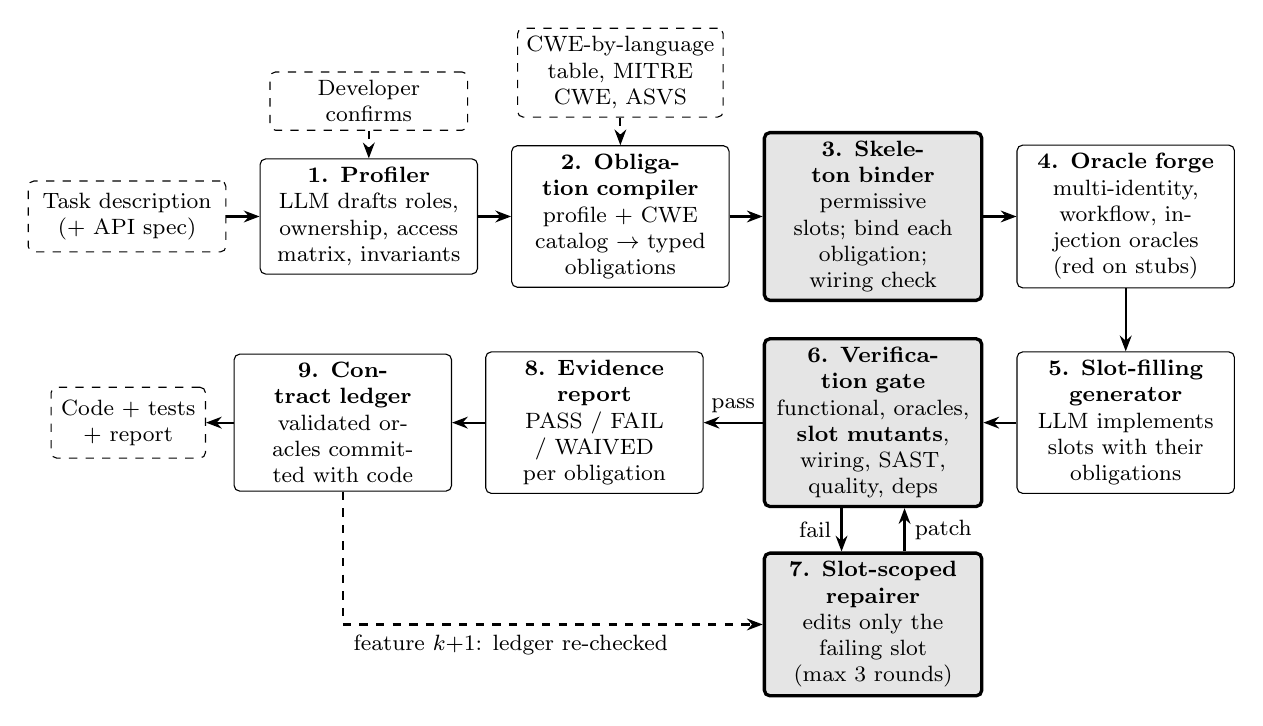
\begin{tikzpicture}[
  font=\footnotesize,
  box/.style={draw, rounded corners=2pt, align=center, minimum height=1.05cm,
              text width=2.55cm, inner sep=3pt},
  core/.style={box, fill=gray!20, very thick},
  io/.style={draw, dashed, rounded corners=2pt, align=center,
             text width=2.3cm, inner sep=3pt, minimum height=0.9cm},
  arr/.style={-{Stealth[length=2mm]}, thick},
  darr/.style={-{Stealth[length=2mm]}, thick, dashed},
  node distance=0.45cm and 0.42cm
]
% Row 1
\node[io] (in) {Task description\\(+ API spec)};
\node[box, right=of in] (prof) {\textbf{1. Profiler}\\LLM drafts roles, ownership, access matrix, invariants};
\node[box, right=of prof] (comp) {\textbf{2. Obligation compiler}\\profile + CWE catalog $\rightarrow$ typed obligations};
\node[core, right=of comp] (bind) {\textbf{3. Skeleton binder}\\permissive slots; bind each obligation; wiring check};
\node[box, right=of bind] (forge) {\textbf{4. Oracle forge}\\multi-identity, workflow, injection oracles (red on stubs)};
% Annotations row 1
\node[io, above=0.35cm of prof, text width=2.3cm, minimum height=0.6cm] (dev) {Developer confirms};
\node[io, above=0.35cm of comp, text width=2.4cm, minimum height=0.6cm] (cat) {CWE-by-language table, MITRE CWE, ASVS};
% Row 2 (right to left)
\node[box, below=0.8cm of forge] (gen) {\textbf{5. Slot-filling generator}\\LLM implements slots with their obligations};
\node[core, left=of gen] (gate) {\textbf{6. Verification gate}\\functional, oracles, \textbf{slot mutants}, wiring, SAST, quality, deps};
\node[core, below=0.55cm of gate] (rep) {\textbf{7. Slot-scoped repairer}\\edits only the failing slot (max 3 rounds)};
\node[box, left=0.75cm of gate] (rept) {\textbf{8. Evidence report}\\PASS / FAIL / WAIVED per obligation};
\node[box, left=of rept] (led) {\textbf{9. Contract ledger}\\validated oracles committed with code};
\node[io, left=0.35cm of led, text width=1.75cm] (out) {Code + tests + report};
% Arrows
\draw[arr] (in) -- (prof);
\draw[arr] (prof) -- (comp);
\draw[arr] (comp) -- (bind);
\draw[arr] (bind) -- (forge);
\draw[arr] (forge) -- (gen);
\draw[arr] (gen) -- (gate);
\draw[arr] (gate) -- node[above]{pass} (rept);
\draw[arr] (rept) -- (led);
\draw[arr] (led) -- (out);
\draw[darr] (dev) -- (prof);
\draw[darr] (cat) -- (comp);
\draw[arr] ([xshift=-4mm]gate.south) -- node[left]{fail} ([xshift=-4mm]rep.north);
\draw[arr] ([xshift=4mm]rep.north) -- node[right]{patch} ([xshift=4mm]gate.south);
\draw[darr] (led.south) |- node[pos=0.7, below]{feature $k{+}1$: ledger re-checked} (rep.west);
\end{tikzpicture}
\caption{Architecture of the proposed framework. Shaded components carry the
novel mechanisms: pre-implementation slot binding, slot-mutation validation of
every oracle, and repair confined to the failing slot. The dashed path shows
the ledger being re-checked when the next feature is added.}
\label{fig:arch}
\end{figure*}

\subsection{Profiler}

The profiler asks an LLM to draft a security context profile $\Pi$ from the
task description and any API specification: roles, resource types,
ownership, the access matrix, and invariants in conditional form. The
developer then confirms or edits a short checklist rather than writing the
profile from scratch. This follows evidence that LLM-only threat elicitation
is incomplete \cite{specdriven2026,threatmodel2026} while human-approved
intent boundaries make downstream verification reliable \cite{autocedar2026}.
The profile is stored as validated YAML so that later stages treat it as
data, not prose. An LLM-only path is kept so that the value of confirmation
can be measured (RQ3).

\subsection{Obligation Compiler}

The compiler deterministically maps profile entries and code features to
obligations. Ownership entries yield object-authorization obligations
(CWE-639/863), role restrictions yield function-authorization obligations
(CWE-862), workflow invariants yield state-transition obligations (CWE-841),
quotas yield rate or limit obligations, and detected sinks yield query,
command and path obligations (for example CWE-89, CWE-78, CWE-22).
Per-language priors come from the weaknesses most frequently observed in the
base study, such as cryptographic and certificate-validation weaknesses in
Java and Python \cite{kharma2026}, and in our measurement, where format-string
and buffer weaknesses dominate C (Section~\ref{sec:rq1}). The compiler uses
rules rather than asking an LLM to predict CWEs, because LLM prediction recall
was 0.448 in prior work \cite{scgagent2025}, and caps each slot at its three
to five relevant obligations, since targeted principles outperformed the full
set in CSDD \cite{csdd2026}.

\subsection{Skeleton Binder}

Before implementation, an LLM proposes a skeleton: routes, function
signatures and named slots such as
\texttt{authz\_booking\_cancel(user, booking)} or
\texttt{guard\_cancel\_transition(booking, now)}. Slots are stubbed
permissively. The binder assigns every obligation to a slot and checks,
by static analysis of the abstract syntax tree, that every route touching a
governed resource calls its bound slots. This wiring check is meant to catch
a failure mode where a guard is defined but never connected to the request
path. Binding before implementation gives the generator a concrete place to
put each defense, which is the sink-grounded guidance the systematization
identified as missing \cite{sok2026}.

\subsection{Oracle Forge}

For every cell of the access matrix and every invariant, the forge
instantiates a deterministic oracle template. Authorization templates use
at least two identities: identity B attempts to read, update or delete a
resource owned by identity A, and the oracle checks observable effects only,
namely the status code, whether A's identifier appears in the response, and
whether A's resource changed. Function-level templates call privileged
operations with an unprivileged role. Workflow templates drive an object
into a forbidden state order. Injection and path templates send payloads to
bound sinks. An LLM fills only request bodies and call sequences; pass and
fail decisions are never made by an LLM. Because slots are permissive, every
oracle must fail on the skeleton before generation; an oracle that passes on
the skeleton is discarded. This avoids trusting self-reported exploit
success, which was invalid in 44--71.5\% of cases in prior work
\cite{pocgym2026}.

\subsection{Slot-Filling Generator}

The generator implements the skeleton. Each slot is presented with only its
bound obligations, expressed as a short contract docstring with
preconditions and the expected sink-specific pattern, such as a
parameterized query or an ownership comparison against the authenticated
identity. Oracles are not shown to the generator, which avoids writing code
to the test. The generator can be any LLM or a coding agent; the framework
only requires that it preserves slot names and signatures.

\subsection{Verification Gate}

The gate runs in a container without network access or version history and
applies nine checks:
G1~functional tests;
G2~contract oracles;
G3~slot mutation, in which each bound slot is replaced by its permissive
mutant (for example an authorization guard that returns true, a dropped
authentication dependency, a parameterized query rewritten as string
formatting, a removed path canonicalization or a deleted state check) and
the corresponding oracle must flip to fail, per (\ref{eq:validity});
G4~wiring, re-running the call-path check so that a guard cannot be removed
or bypassed;
G5~static analysis with Semgrep and Bandit or CodeQL;
G6~quality with a linter and complexity metrics;
G7~dependency existence in the package registry and known-vulnerability
checks;
G8~secret scanning; and
G9~integrity, in which oracle files are hash-locked so that any skip,
deletion or edit by the generator fails the task.
G3 is the key addition. It turns ``the tests passed'' into ``the tests
passed and are capable of failing,'' reusing the contrastive principle of
AutoBaxBuilder \cite{autobax2025} and the logic of mutation testing
\cite{jia2011} without needing a reference solution.

\subsection{Slot-Scoped Repairer}

When an oracle fails, the repairer maps it to its obligation and slot and
gives the model only three inputs: the body of that slot, the obligation
text, and the failing request and response trace. A patch is rejected if any
changed line falls outside the slot's source span, if it removes a guard or
breaks the wiring check, or if it breaks functional tests or previously
passing oracles. Repair stops after three rounds, consistent with reports
that feedback gains taper after three to four iterations \cite{blyth2025}.
Confining repair by location rather than by diff size distinguishes this
step from diff budgets \cite{scaffold2026} and from whole-module repair
\cite{testsasspec2026}, and it removes the opportunity to ``fix'' a failure
by deleting unrelated functionality \cite{dai2025}.

\subsection{Evidence Report and Contract Ledger}

The evidence report lists every obligation with its status, slot location,
oracle, whether the mutant was killed, and any static or quality findings,
in Markdown and in SARIF so that it appears in pull-request review. A
reviewer needs to read only WAIVED and FAIL entries and changes outside
bound slots. The ledger commits validated oracles and bindings with the
code. When the next feature is requested, the profiler, compiler and binder
run on the change only, and every oracle already in the ledger must remain
valid; defense survival (\ref{eq:ds}) measures how often it does. In agent
workflows the ledger can run as a pre-commit or tool hook.

\begin{algorithm}[t]
\caption{The proposed framework for one feature step $k$}
\label{alg:cg}
\begin{algorithmic}[1]
\REQUIRE task $t_k$, program $P_{k-1}$, ledger $L_{k-1}$
\STATE $\Pi \leftarrow$ \textsc{Confirm}(\textsc{DraftProfile}($t_k$))
\STATE $C \leftarrow$ \textsc{Compile}($\Pi$, CWE catalog)
\STATE $(S, \beta) \leftarrow$ \textsc{Bind}($C$, $P_{k-1}$); require well-formed $\beta$
\STATE $\Omega \leftarrow \{\omega_o \leftarrow \textsc{Forge}(o) : o \in C\}$; drop $\omega_o$ with $\omega_o(S) = \mathit{pass}$
\STATE $P \leftarrow$ \textsc{Generate}($S$, $C$)
\FOR{$r = 0$ \TO $3$}
  \STATE $F \leftarrow \{o : \omega_o(P) = \mathit{fail}\} \cup \{o \in L_{k-1} : \omega_o \text{ not valid on } P\}$
  \IF{$F = \emptyset$ \OR $r = 3$}
    \STATE \textbf{break}
  \ENDIF
  \FORALL{$o \in F$}
    \STATE $\delta \leftarrow$ \textsc{Repair}($\beta(o)$, $o$, trace)
    \IF{$\delta$ admissible}
      \STATE $P \leftarrow P \oplus \delta$
    \ENDIF
  \ENDFOR
\ENDFOR
\FORALL{$o \in C$}
  \STATE status$(o) \leftarrow$ PASS if $\omega_o$ valid on $P$ (\ref{eq:validity}); FAIL if $\omega_o(P) = \mathit{fail}$; else WAIVED
\ENDFOR
\STATE $L_k \leftarrow L_{k-1} \cup \{\omega_o : \text{status}(o) = \text{PASS}\}$
\RETURN $P$, report, $L_k$
\end{algorithmic}
\end{algorithm}

\subsection{Worked Example}

Consider a booking service. The developer confirms one access-matrix row, ``a
member may cancel only their own booking; an administrator may cancel any
booking,'' and one invariant, ``if a booking is not confirmed or its start
time has passed, the system shall reject cancellation.'' The compiler emits
obligation $o_7$ (object authorization, CWE-639/863, MUST, multi-identity
replay) and $o_8$ (state transition, CWE-841, MUST, workflow-order test).
The binder creates \texttt{authz\_booking\_cancel} and
\texttt{guard\_cancel\_transition}, both permissive, and confirms that the
cancel route calls both. The forge produces two oracles: member B attempts to
cancel member A's booking and must receive a denial with A's booking
unchanged, and a cancellation after the start time must be rejected. Both
fail on the skeleton. Once generation makes both pass, the gate replaces
\texttt{authz\_booking\_cancel} with a function that returns true; if the
$o_7$ oracle does not fail, it is vacuous and $o_7$ is reported WAIVED, not
PASS. If the $o_8$ oracle fails, only \texttt{guard\_cancel\_transition} and
the failing trace are sent to the repairer. When a later feature adds
rescheduling, both oracles remain in the ledger and must stay valid.

\subsection{Planned Implementation}

The framework will be implemented in Python for FastAPI services. Profiles
and contracts will use YAML validated with Pydantic; the binder and wiring
check will use Python's abstract syntax tree tooling; oracles will use pytest
with FastAPI's test client; mutants will be produced by rewriting slot
bodies; static and quality checks will use Semgrep, Bandit, CodeQL, Ruff and
radon; dependency checks will use the package registry and vulnerability
databases; and the gate will run in a container. Model access will go through
a provider-independent client so that hosted models and a local open-weight
coder can be swapped; the measurement in Section~\ref{sec:rq1} already uses
such a client. Oracle templates for multi-identity authorization require no
LLM, which keeps the method affordable.

%==========================================================================
\section{Evaluation Plan (RQ2--RQ6)}
\label{sec:plan}
%==========================================================================

This section fixes the evaluation design in advance; its results will be
reported in follow-up work.

\subsection{Benchmarks}

\textbf{BaxBench subset.} Python-framework scenarios from BaxBench
\cite{baxbench2025}, prioritizing scenarios whose expert exploits cover
access-control weaknesses. Exploits serve as held-out security tests.

\textbf{CWEval subset.} Python tasks from CWEval \cite{cweval2025}, which
supply executable functional and security tests at function level, where
bindings attach mostly to sinks rather than to authorization.

\textbf{Custom authorization services.} Ten to fifteen small FastAPI
services, such as bookings, multi-tenant notes, orders with refunds and
document sharing, each with an access matrix, workflow invariants and a
hidden security suite written by a team member who does not write the oracle
templates. Tasks will be written after the evaluated models' training
cut-offs.

\textbf{Feature sequences.} Each custom service will be extended over four to
five feature turns covering expansion, editing and refactoring, following
the taxonomy of MT-Sec \cite{mtsec2025}, with code supplied to the model as
diffs.

\subsection{Models}

RQ2--RQ6 will use two of the five measurement models and one local
open-weight coding model, so that results cover both hosted and self-hosted
settings and show where the method stops helping weaker models.

\subsection{Baselines}

All baselines will use the same model, the same sandbox and the same cap on
model calls and tokens.
B0~direct generation.
B1~a generic security reminder.
B2~MA-CoT-style prompting with retrieved CWE mitigations \cite{macot2026}.
B3~profile-conditioned specification without binding, in the style of
\cite{specdriven2026}, with an ASVS-only variant.
B4~the framework's own validated oracles given upfront as a specification,
with whole-module repair \cite{testsasspec2026}; this isolates the effect of
binding and slot-scoped repair from simply having good tests.
B5~an open-source coding agent that may run functional tests and write its
own tests, the strongest generic baseline \cite{sok2026}.
B6~an SCGAgent-style loop of self-generated tests and CWE guidelines
\cite{scgagent2025}.
B7~anchor and diff-budget repair approximating SCAFFOLD-CEGIS
\cite{scaffold2026}, with budgets declared in advance.
B8~a static-analysis feedback loop \cite{blyth2025}.

\subsection{Metrics and Ablations}

Every table will report pass@1, secure-pass@1 and secure@pass together, plus
production-ready@1, contract coverage, oracle adequacy, waive rate, defense
survival, the review-effort proxy, and cost in tokens, calls and wall-clock
time (Section~IV). Ablations remove one mechanism at a time: binding
(contract as a prose checklist), mutation validation (oracles trusted as
generated), slot-scoped repair (whole-file repair), the business profile
(CWE obligations only), the CWE catalog (profile obligations only), and the
ledger. Two further comparisons contrast LLM-generated with deterministic
authorization oracles, and LLM-only with developer-confirmed profiles. The
binding ablation and the comparison with B4 are decisive: if binding adds
nothing over the same validated oracles given upfront, the remaining
contributions are the validated oracles and the defense-survival protocol,
and we will report that outcome as such.

\subsection{Validity Protocol}

The sandbox will have no network and no version history, and all tool calls
will be logged. Held-out tests never appear in any prompt. Oracle files are
hash-locked. Oracle templates and hidden suites have different authors. Every
configuration will run with at least three seeds; we will report bootstrap
95\% confidence intervals and compare paired outcomes with McNemar's test and
Holm correction. A random 10\% of secure verdicts will be audited manually.
Generation failures count as failures. Quality thresholds and repair budgets
will be fixed before the main runs. The measurement in
Section~\ref{sec:rq1} already applies the same snapshot hashing, sandboxing
and paired statistics.

%==========================================================================
\section{Threats to Validity}
%==========================================================================

\subsection{Updated Measurement (RQ1)}

\textbf{Construct validity.} Scanner hits from Semgrep, Bandit and
Flawfinder are potential findings, not confirmed vulnerabilities, and static
tools are imperfect measures of security \cite{tessa2026,sastlabels2026}; we
therefore report the share of artifacts with a finding, not a secure rate.
The triage labels, and the review of functional oracles and adapters, were
proposed with AI assistance and must be confirmed by the authors before
publication. CodeQL and SonarQube, which the base study used, were not run, so
RQ1 security results are not directly comparable with the base study's, and
the functional tests cover only 16.2\% of combinations. Compilation is never
treated as correctness.

\textbf{Internal validity.} Each combination received one sample at
temperature 0.2 with our own prompt, so sampling variance is not captured.
The comparison with the base study's outputs confounds models with prompt,
temperature, token limits, extraction, generation dates and undocumented
post-processing of the published files; it is descriptive only.

\textbf{External validity.} The 40 tasks were chosen by judgment, so each
model and language cell rests on 40 tasks with wide intervals, and the four
language cells of a task are correlated although the paired tests treat them
as independent. The five models were chosen for low price but are not matched
in size or price: Gemini 3.8 Flash and Mistral Large 4 cost several times more
per output token than the other three, so differences between providers may
partly reflect model size, and providers may update a model behind the same
identifier. A disjoint 10-task check reproduced the main language pattern.

\subsection{Planned Framework Evaluation}

\textbf{Internal validity.} A framework that writes its own tests risks
grading itself. The design separates the two roles: the framework's oracles
drive generation and repair, but every reported security result will come
from held-out exploits or hidden suites written by a different author, and
those are never shown to any system. Oracles may also reject correct code;
this false-fail rate will be measured by running every oracle on
reference-secure solutions. Results from agents vary between runs, and
published agent results have shifted by several points on re-runs
\cite{endor2026}, so every configuration will use at least three seeds and
paired statistical tests. Contamination and shortcutting are limited by
writing custom tasks after the models' training cut-offs and by removing
network access and version history from the sandbox. The developer
confirmation step is a potential weak point, since people tend to accept
plausible but wrong LLM suggestions; the LLM-only profile ablation measures
how much the result depends on it.

\textbf{Construct validity.} Slot mutation shows that an oracle can detect
the \emph{absence} of a defense, because the permissive mutant removes the
check entirely. It does not show that the check is correct for every input:
an oracle could kill the permissive mutant yet miss a partially wrong guard,
for example one that checks the role but not ownership. Richer mutation
operators, such as partial-guard and off-by-one-state mutants, would tighten
this and are left to future work. The review-effort measure is a proxy, the
number of items a reviewer must inspect, and not measured human effort; any
claim about effort reduction will be limited to that proxy unless a user
study is added.

\textbf{External validity.} The dynamic oracle layer targets Python and
FastAPI services, and the custom tasks are small services rather than large
repositories; results may not transfer to other frameworks, to languages
without comparable test tooling, or to repository-scale changes. The
multi-language evidence in this paper comes from the RQ1 measurement, which
uses static tools and a small functional subset only. Method effects can
depend on the model: a prior test-and-guideline loop helped one model and
hurt others \cite{scgagent2025}, so the evaluation includes a local
open-weight model to show where the method stops helping.

\textbf{Novelty.} The field is moving quickly, and several 2026 preprints on
LLM-guided risk analysis and agent test generation were available only as
titles during our literature search. Our novelty claim is limited to the
combination of pre-implementation slot binding with slot-mutation oracle
validation, slot-scoped repair and an executable regression ledger, to the
best of our knowledge as of October 2026.

%==========================================================================
\section{Conclusion and Future Work}
%==========================================================================

Our updated measurement of five current lower-cost models on 800
combinations shows that three quarters of outputs compile, that most losses
come from empty or truncated responses rather than from invalid code, that
language matters more than model, and that the tests and scanners available
for this code say little about whether it enforces its security
requirements: the approved functional tests covered 16.2\% of combinations
and checked no security property, and scanner hits concentrate in C library
calls while missing authorization produces no hit at all. Together with prior
evidence that LLMs know secure-coding rules but fail to place the defense
where it belongs and that defenses erode as code evolves, this motivates the
framework proposed here. It compiles CWE knowledge and developer-confirmed
business rules into obligations, binds each obligation to a named slot before
implementation, trusts a security oracle only when it fails on a weakened
version of its own slot, confines repair to the failing slot, and keeps
validated oracles as a ledger that later features must satisfy. For a
developer, the intended result is a short list of what was proven, what
failed, and what still needs human judgement, rather than an unverified body
of generated code.

The next step is to implement the framework and run the evaluation fixed in
Section~\ref{sec:plan}, which will answer RQ2--RQ6. Further directions
follow. First, the framework would produce training data that prior
secure-code training methods lack: slot repairs labelled by executable,
validated oracles. Reviewed training methods derive their security signal
from static analyzers or teacher models \cite{srcode2026,secvec2026}; using
oracle-labelled repairs for supervised and preference fine-tuning of a small
open model is a natural later phase. Second, richer mutation operators would
strengthen what a passing oracle certifies. Third, expressing the access
matrix in an established policy language would let the same profile drive
both application oracles and policy verification \cite{autocedar2026}.
Fourth, the ledger can run as a hook inside coding agents, which would allow
a study of defense survival in real multi-turn agent sessions. Finally, a
controlled study with developers would test whether the evidence report
reduces review time, not only the number of items to inspect.

% TODO(authors): add an Acknowledgment section if needed; it was empty.

%==========================================================================
% TODO(authors): references marked "TODO" below are incomplete. Look up each
% arXiv ID and fill in the exact title and full author list before submission.
\begin{thebibliography}{00}

\bibitem{kharma2026} M. F. Kharma, S. Choi, M. Alkhanafseh, and D. Mohaisen,
``Security and quality in LLM-generated code: A multi-language, multi-model
analysis,'' \textit{IEEE Trans. Dependable Secure Comput.}, vol. 23, no. 3,
pp. 7300--7314, May/Jun. 2026, doi: 10.1109/TDSC.2026.3672745.

\bibitem{perry2023} N. Perry, M. Srivastava, D. Kumar, and D. Boneh, ``Do
users write more insecure code with AI assistants?'' in \textit{Proc. ACM
SIGSAC Conf. Comput. Commun. Secur. (CCS)}, Copenhagen, Denmark, Nov. 2023,
doi: 10.1145/3576915.3623157.

\bibitem{metr2025} J. Becker, N. Rush, B. Barnes, and D. Rein, ``Measuring
the impact of early-2025 AI on experienced open-source developer
productivity,'' 2025, arXiv:2507.09089.

\bibitem{susvibes2026} S. Zhao, D. Wang, K. Zhang, J. Luo, Z. Li, and L. Li,
``Is vibe coding safe? Benchmarking vulnerability of agent-generated code in
real-world tasks,'' in \textit{Proc. 43rd Int. Conf. Mach. Learn. (ICML)},
PMLR vol. 306, pp. 162269--162292, Jul. 2026.

\bibitem{baxbench2025} M. Vero, N. M\"{u}ndler, V. Chibotaru, V. Raychev,
M. Baader, N. Jovanovi\'{c}, J. He, and M. Vechev, ``BaxBench: Can LLMs
generate correct and secure backends?'' in \textit{Proc. 42nd Int. Conf.
Mach. Learn. (ICML)}, PMLR vol. 267, pp. 61344--61390, Jul. 2025.

\bibitem{sok2026} R. Patir, K. Guo, H. Cai, and H. Hu, ``SoK: AI secure code
generation: Progress, pitfalls, and paths forward,'' 2026, arXiv:2606.25195.

% TODO: authors, venue and year missing.
\bibitem{securecoder2026} ``Towards secure code generation with LLMs: A study
on Common Weakness Enumeration.''

\bibitem{macot2026} M. F. Kharma, M. Alkhanafseh, A. Sabbah, and
D. Mohaisen, ``Enhancing reliability in LLM-based secure code generation,''
2026, arXiv:2605.24300.

\bibitem{csdd2026} S. R. Marri, ``Constitutional spec-driven development:
Enforcing security by construction in AI-assisted code generation,'' 2026,
arXiv:2602.02584.

\bibitem{tessa2026} M. Tessa, I. E. Olatunji, A. War, J. Klein, and
T. F. Bissyand\'{e}, ``How secure is secure code generation? Adversarial
prompts put LLM defenses to the test,'' 2026, arXiv:2601.07084.

\bibitem{mtsec2025} R. Rawal, J. Y. F. Chiang, C. Shen, J. S. Tian,
A. Mahajan, T. Goldstein, and Y. Chen, ``Benchmarking correctness and
security in multi-turn code generation,'' in \textit{NeurIPS 2025 Workshop on
Multi-Turn Interactions in Large Language Models}, 2025, arXiv:2510.13859.

\bibitem{scaffold2026} Y. Chen, Y. Bian, H. Wang, S. Li, and Z. Cui,
``SCAFFOLD-CEGIS: Preventing latent security degradation in LLM-driven
iterative code refinement,'' 2026, arXiv:2603.08520.

\bibitem{specdriven2026} O. Grynets, O. Kaskun, A. Salyk, D. Zhuravchak, and
V. Lyashkevych, ``Specification-driven development benchmark: Security
knowledge transition,'' 2026, arXiv:2606.00167.

\bibitem{dai2025} S.-C. Dai, J. Xu, and G. Tao, ``Rethinking the evaluation
of secure code generation,'' in \textit{Proc. IEEE/ACM 48th Int. Conf. Softw.
Eng. (ICSE)}, Rio de Janeiro, Brazil, Apr. 2026,
doi: 10.1145/3744916.3773217.

\bibitem{meyer1992} B. Meyer, ``Applying `design by contract','' \textit{Computer},
vol. 25, no. 10, pp. 40--51, Oct. 1992.

\bibitem{cweval2025} J. Peng, L. Cui, K. Huang, J. Yang, and B. Ray,
``CWEval: Outcome-driven evaluation on functionality and security of LLM
code generation,'' in \textit{Proc. IEEE/ACM Int. Workshop Large Lang. Models
Code (LLM4Code)}, 2025, arXiv:2501.08200.

\bibitem{endor2026} Endor Labs, ``Agent Security League: Evaluating the
security of AI-coded software,'' 2026. [Online]. Available:
https://www.endorlabs.com/learn/agent-security-league-evaluating-the-security-of-ai-coded-software

% TODO: exact title and authors missing (title below is a placeholder).
\bibitem{sastlabels2026} ``[Reliability of SAST tools as evaluation oracles for
LLM-generated code],'' in \textit{SANER Workshops}, 2026, arXiv:2602.05868.

% TODO: authors missing.
\bibitem{brace2026} ``Activating latent security knowledge through LLM-guided
risk analysis for secure code generation,'' 2026, arXiv:2606.16244.

\bibitem{scgagent2025} R. Saul, H. Wang, K. Sen, and D. Wagner, ``SCGAgent:
Recreating the benefits of reasoning models for secure code generation with
agentic workflows,'' 2025, arXiv:2506.07313.

\bibitem{testsasspec2026} Y. Liang, C. Gan, R. Ying, H. Wei, Z. Cui, and
S. Ni, ``Security tests as executable specifications for LLM code generation:
Benefits, trade-offs, and coverage limits,'' 2026, arXiv:2608.09740.

% TODO: exact title and full author list missing (title is a placeholder).
\bibitem{blyth2025} Blyth \textit{et al.}, ``[Static analysis as a feedback
loop for LLM-generated code],'' 2025, arXiv:2508.14419.

\bibitem{pocgym2026} D. Gezgin, A. Das, S. Kim, Z. Huang, N. Stojkovic, and
C. Wang, ``PoC-Gym: Towards more reliable LLM-assisted proof-of-concept
exploit generation,'' in \textit{2nd Workshop on LLMs for Generative Software
Engineering (LLM4SE) at STAF}, Rennes, France, 2026, arXiv:2602.04165.

\bibitem{autobax2025} T. von Arx, N. M\"{u}ndler, M. Vero, M. Baader, and
M. Vechev, ``AutoBaxBuilder: Bootstrapping code security benchmarking,'' in
\textit{Proc. 43rd Int. Conf. Mach. Learn. (ICML)}, PMLR vol. 306,
pp. 3905--3952, Jul. 2026.

% TODO: exact title and authors missing (title is a placeholder).
\bibitem{threatmodel2026} ``[LLM-based STRIDE threat classification],'' 2026,
arXiv:2605.10808.

\bibitem{autocedar2026} A. Vatsa, S. Shome, Y. Zhou, and W. Eiers,
``AutoCedar: An agentic framework for verifier-guided access control policy
synthesis,'' 2026, arXiv:2607.03656.

\bibitem{authprobe2026} J. Barach, ``AuthProbe: Specification-driven,
multi-identity detection of broken object-level authorization in
recruitment APIs,'' 2026, arXiv:2607.20574.

% TODO: authors missing.
\bibitem{evocode2026} ``EvoCode-Bench: Evaluating coding agents in multi-turn
iterative interactions,'' 2026, arXiv:2605.24110.

\bibitem{srcode2026} J. Quan, X. Li, B. Wang, G. An, L. Liu, D. Huang,
L. Lin, and C. Hou, ``Learning to generate secure code via token-level
rewards,'' 2026, arXiv:2602.23407.

% TODO: authors missing.
\bibitem{secvec2026} ``Functional and secure code generation with task
vectors,'' 2026, arXiv:2607.07881.

% TODO: authors missing.
\bibitem{codeguardplus2024} ``Constrained decoding for secure code
generation,'' 2024, arXiv:2405.00218.

\bibitem{jia2011} Y. Jia and M. Harman, ``An analysis and survey of the
development of mutation testing,'' \textit{IEEE Trans. Softw. Eng.}, vol. 37,
no. 5, pp. 649--678, 2011.

\bibitem{wilson1927} E. B. Wilson, ``Probable inference, the law of
succession, and statistical inference,'' \textit{J. Amer. Statist. Assoc.},
vol. 22, no. 158, pp. 209--212, 1927.

\bibitem{mcnemar1947} Q. McNemar, ``Note on the sampling error of the
difference between correlated proportions or percentages,''
\textit{Psychometrika}, vol. 12, no. 2, pp. 153--157, 1947.

\bibitem{holm1979} S. Holm, ``A simple sequentially rejective multiple test
procedure,'' \textit{Scand. J. Statist.}, vol. 6, no. 2, pp. 65--70, 1979.

\bibitem{newcombe1998} R. G. Newcombe, ``Improved confidence intervals for
the difference between binomial proportions based on paired data,''
\textit{Statist. Med.}, vol. 17, no. 22, pp. 2635--2650, 1998.

\end{thebibliography}

\end{document}
